\section{Introduction}
Ultra-fine entity typing (UFET) \cite{ufet} aims to predict extremely fine-grained types ({\it e.g., president, politician}) of a given entity mention within its context. It provides detailed semantic understandings of entity mention and is a fundamental step in fine-grained named entity recognition \cite{fget}, and can be utilized to assist various downstream tasks such as relation extraction \cite{fewrel}, keyword extraction \cite{huang2020ner} and content recommendation \cite{upadhyay2021explainable}.

\begin{figure}
    \centering
    \scalebox{0.3}{
    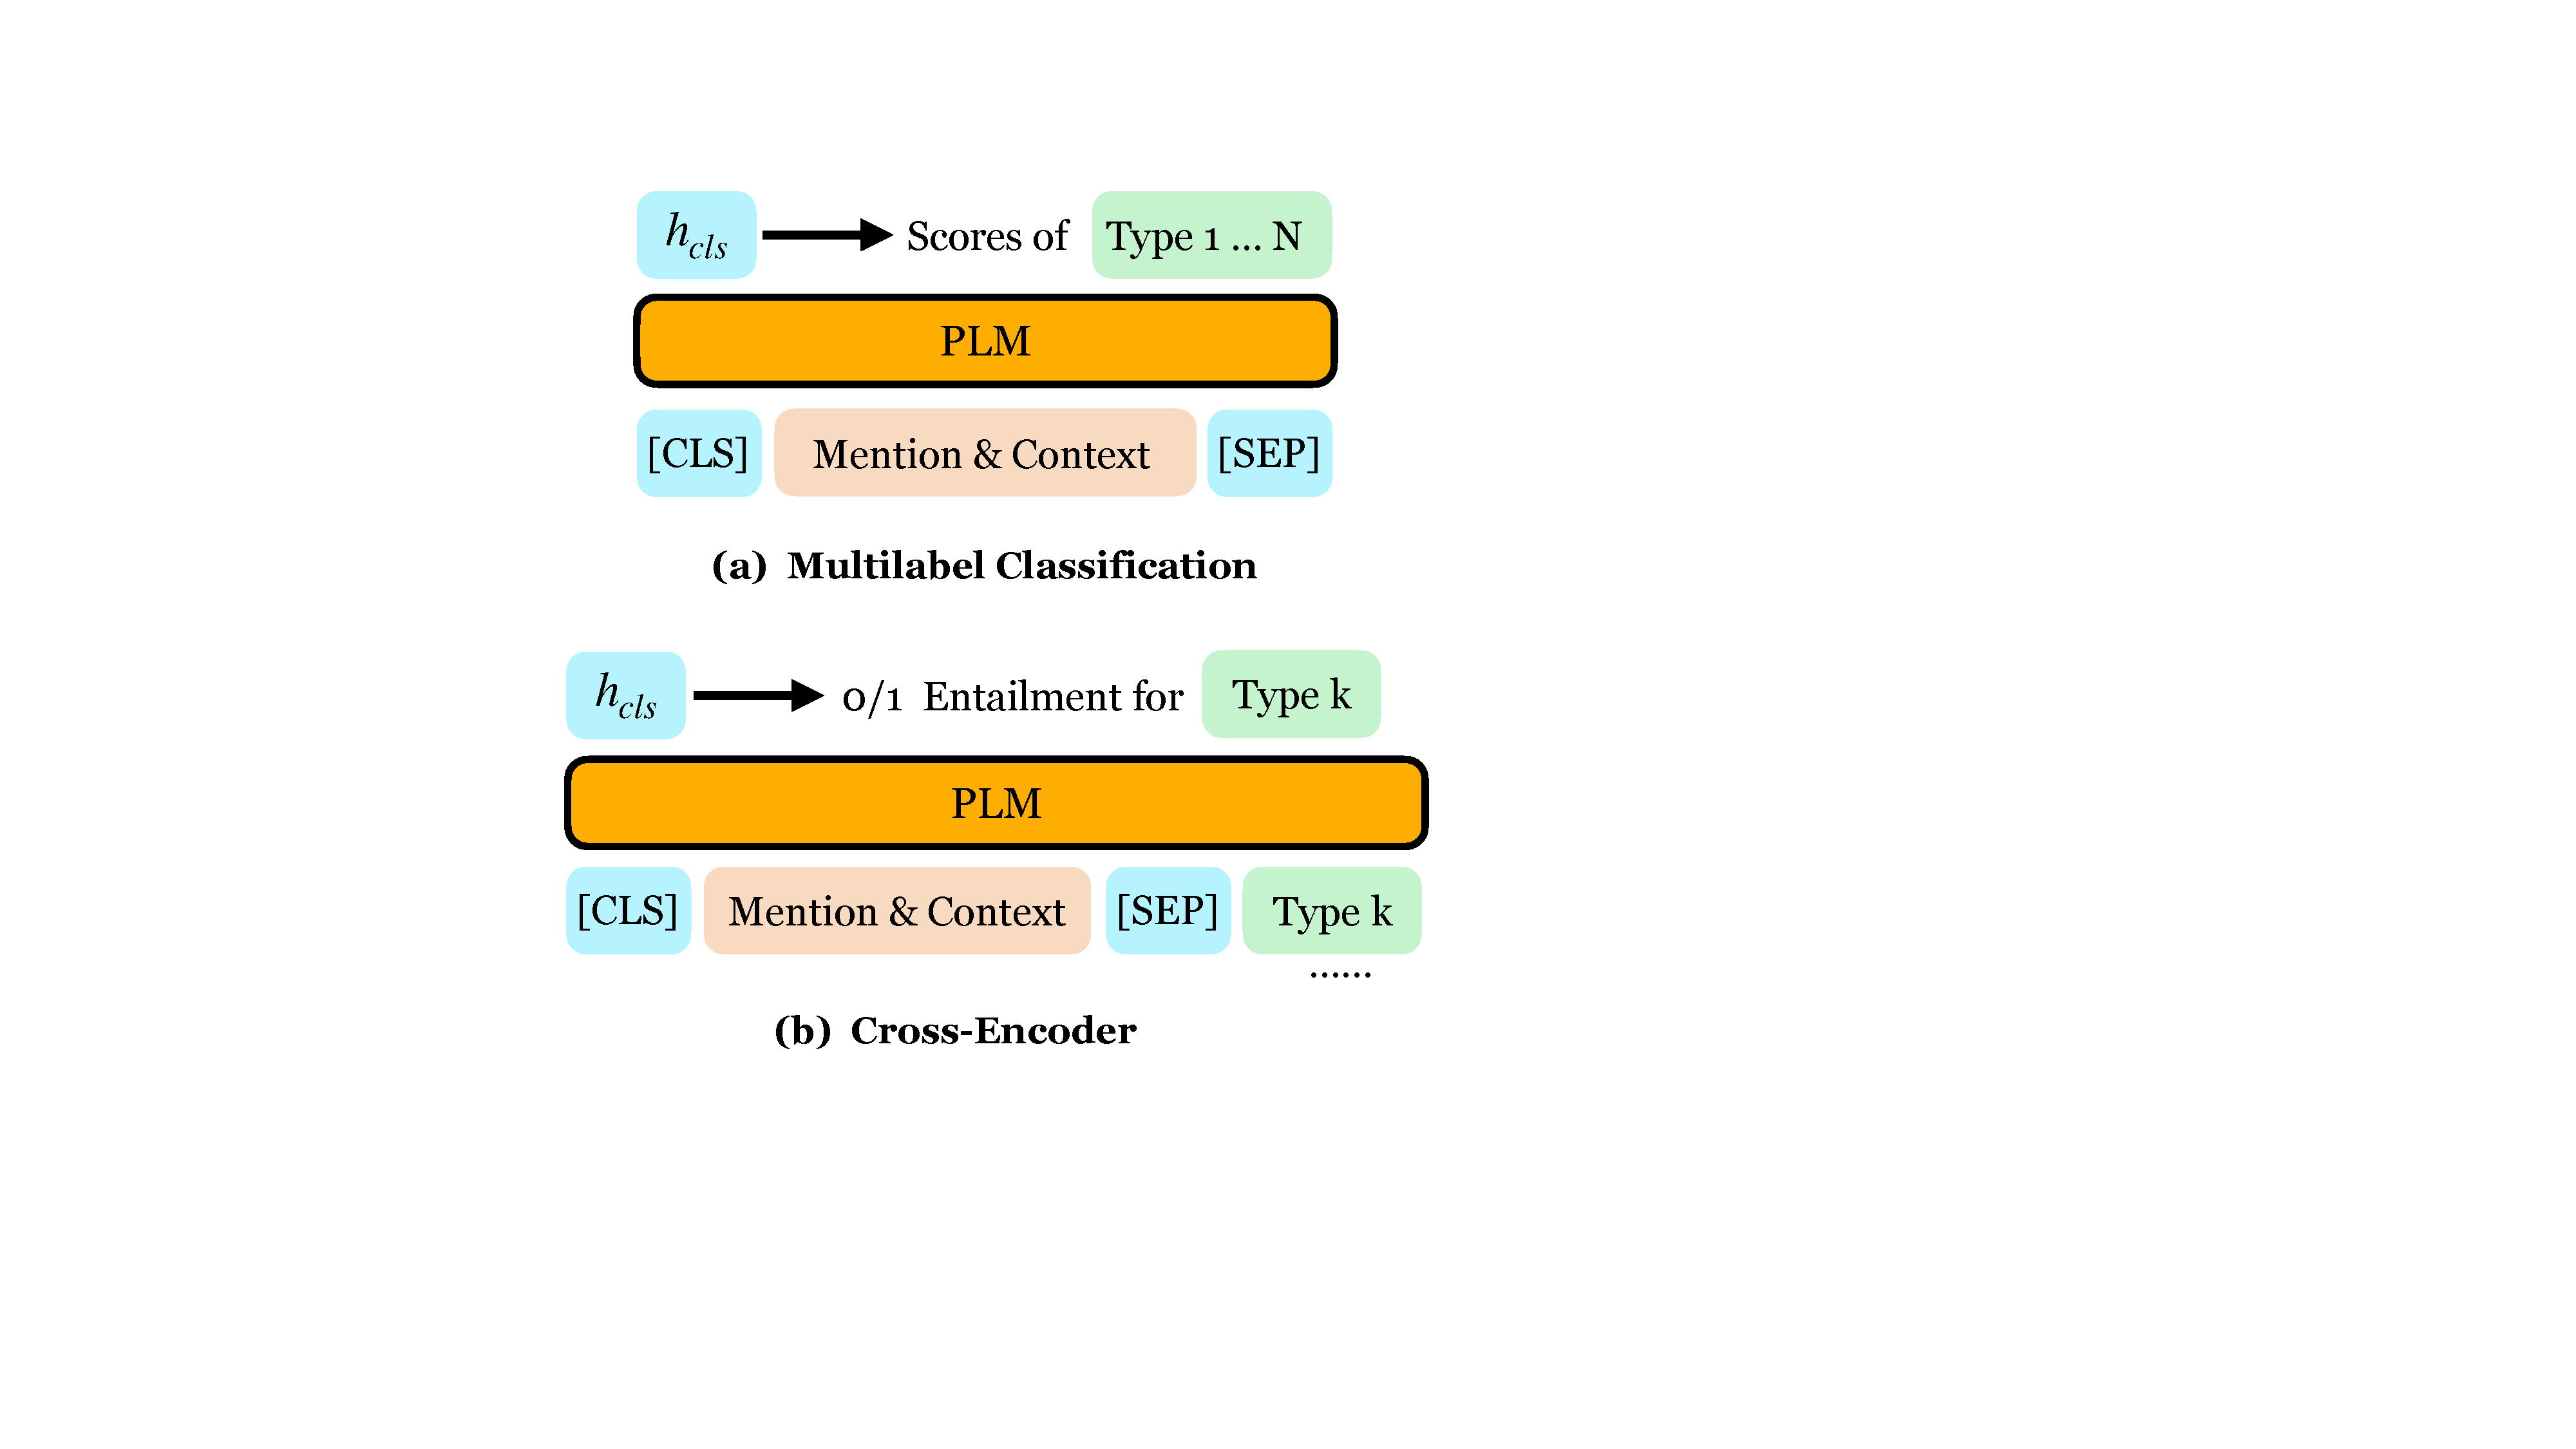
\includegraphics{src/img/mlc_ce.pdf}}
    \caption{Cross-Encoder and multi-label classification.}
    \label{fig:mlc_ce}
\end{figure}

\begin{figure*}[t]
    \centering
    \scalebox{0.28}{
    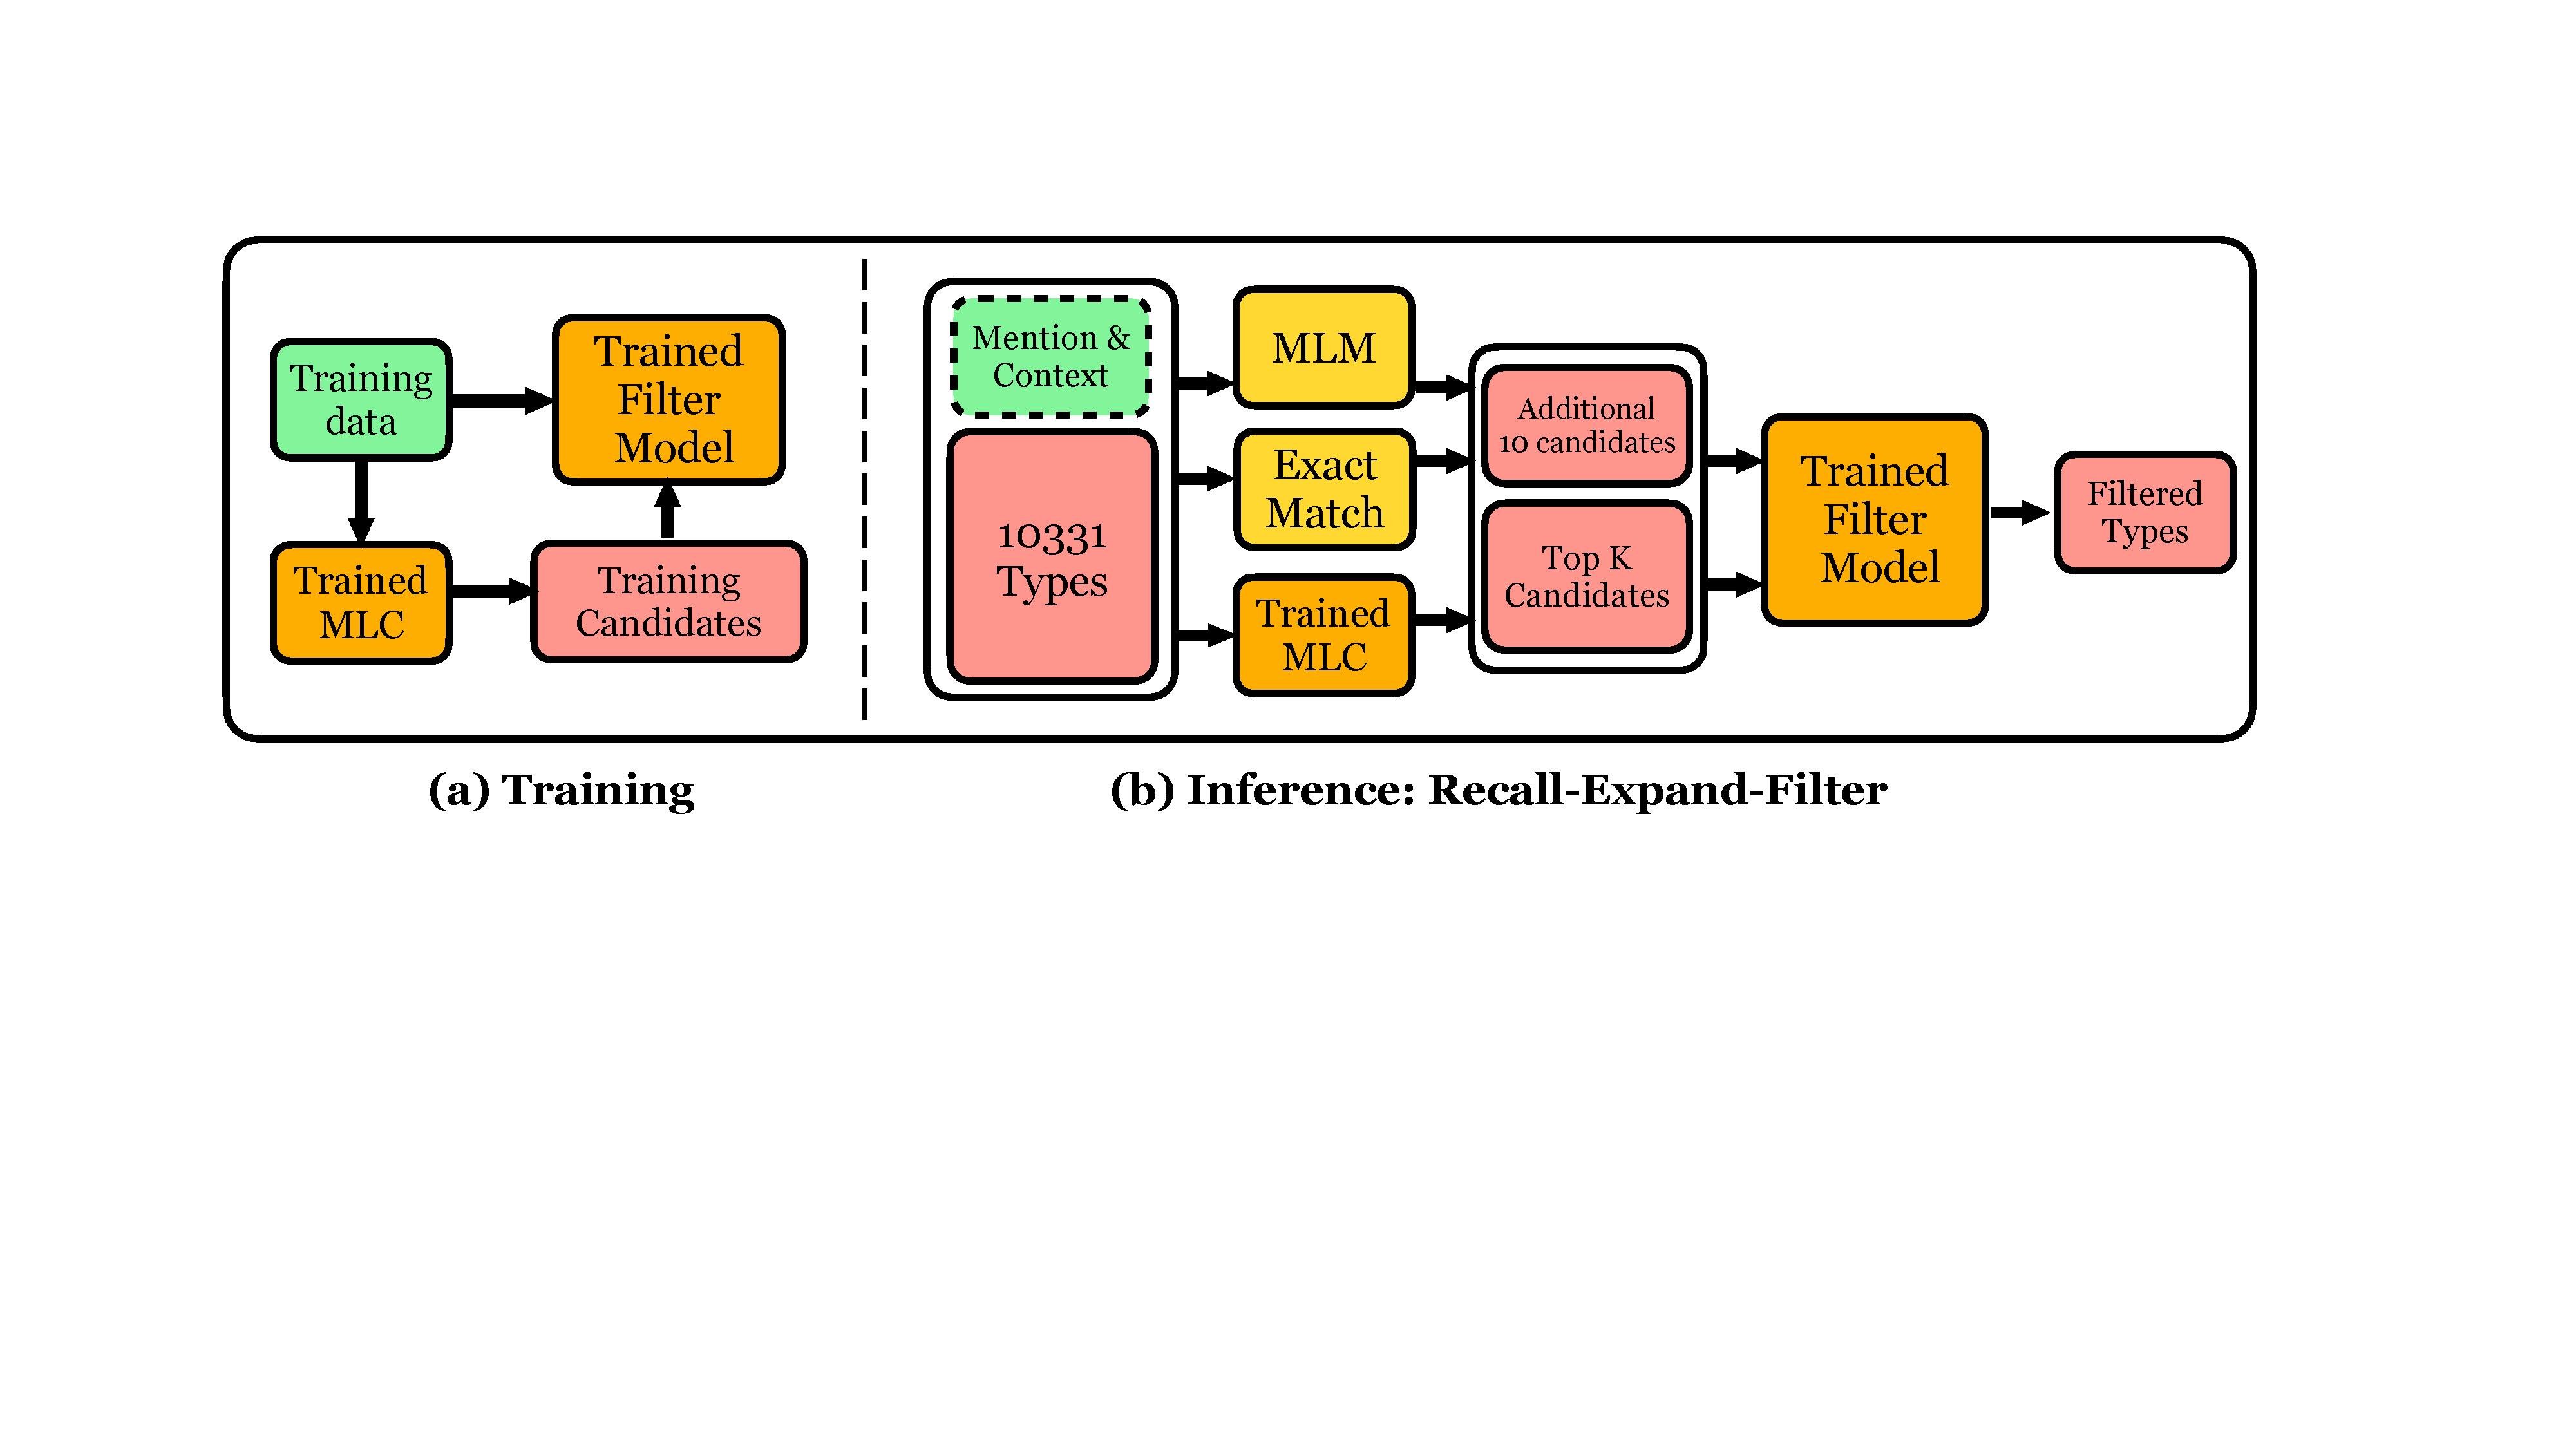
\includegraphics{src/img/paradigm.pdf}}
    \caption{Training and inference of the recall-expand-filter pradigm.}
    \label{fig:paradigm}
\end{figure*}

Most recently, the cross-encoder (CE) based method \cite{lite} achieves the SOTA performance in UFET. Specifically, \citet{lite} proposed to treat the mention with its context as a premise, and each ultra-fine-grained type as a hypothesis. They then concatenate them together as input and feed it into a pretrained language model (PLM) (e.g., RoBERTa \cite{liu2019roberta}) to score the entailment of mention-type pair as illustrated in Figure \ref{fig:mlc_ce}(b). Compared to the traditional multi-label classification method (shown in Figure \ref{fig:mlc_ce}(a)) that simultaneously scores all types using the mention representation, CE incorporates type semantics in the inference process and enables deeper interactions between types and mention to achieve better performance. However, the CE architecture is slow in inference because it has to enumerate all types (up to 10$k$ types) and score entailment of them given the mention as a premise. There is also no direct interaction between types in CE and is therefore unable to model correlations between types (e.g., one has to be a person if he or she is categorized as a politician), which has been proved to be useful in previous works \cite{npcrf, xiong-etal-2019-imposing}.

To this end, we propose a recall-expand-filter Paradigm for UFET (illustrated in Figure \ref{fig:paradigm}) and a novel model called {\bf \textsc{\name}} for faster and more accurate ultra-fine entity typing. As the name suggests, we first train a multi-label classification (MLC) model to efficiently \textbf{recall} top $K$ candidate types which reduce the number of potential types from thousands to hundreds. As the MLC model recalls candidates based on representations learned from the training data, it's hard to recall candidates that are scarce or unseen in the training set. To this end, we apply a multi-way type candidate \textbf{expansion} step utilizing lexical information and weak supervision from masked language models \cite{mlmet} to improve the recall rate of the candidate set. Last but not least, we propose a backbone called multi-candidate cross-encoder ({\bf \textsc{\name}}) to concurrently encode and \textbf{filter} the expanded type candidate set. Different from CE,  ({\bf \textsc{\name}}) concatenates all recalled type candidates to the mention and its context. The concatenated input is then fed into a PLM to obtain candidate representations and candidate scores. The {\bf \textsc{\name}} architecture allows us to infer types simultaneously from the candidate set while preserving the advantages of CE. Concatenating all candidates also enables {\bf \textsc{\name}} implicitly learns the correlation between types. The advantages of {\bf \textsc{\name}} over existing architectures are shown in Figure \ref{fig:adv}. We also comprehensively investigate the performance and efficiency of {\bf \textsc{\name}} with different input formats and attention mechanisms.

\begin{figure}[t]
    \centering
    \scalebox{0.22}{
    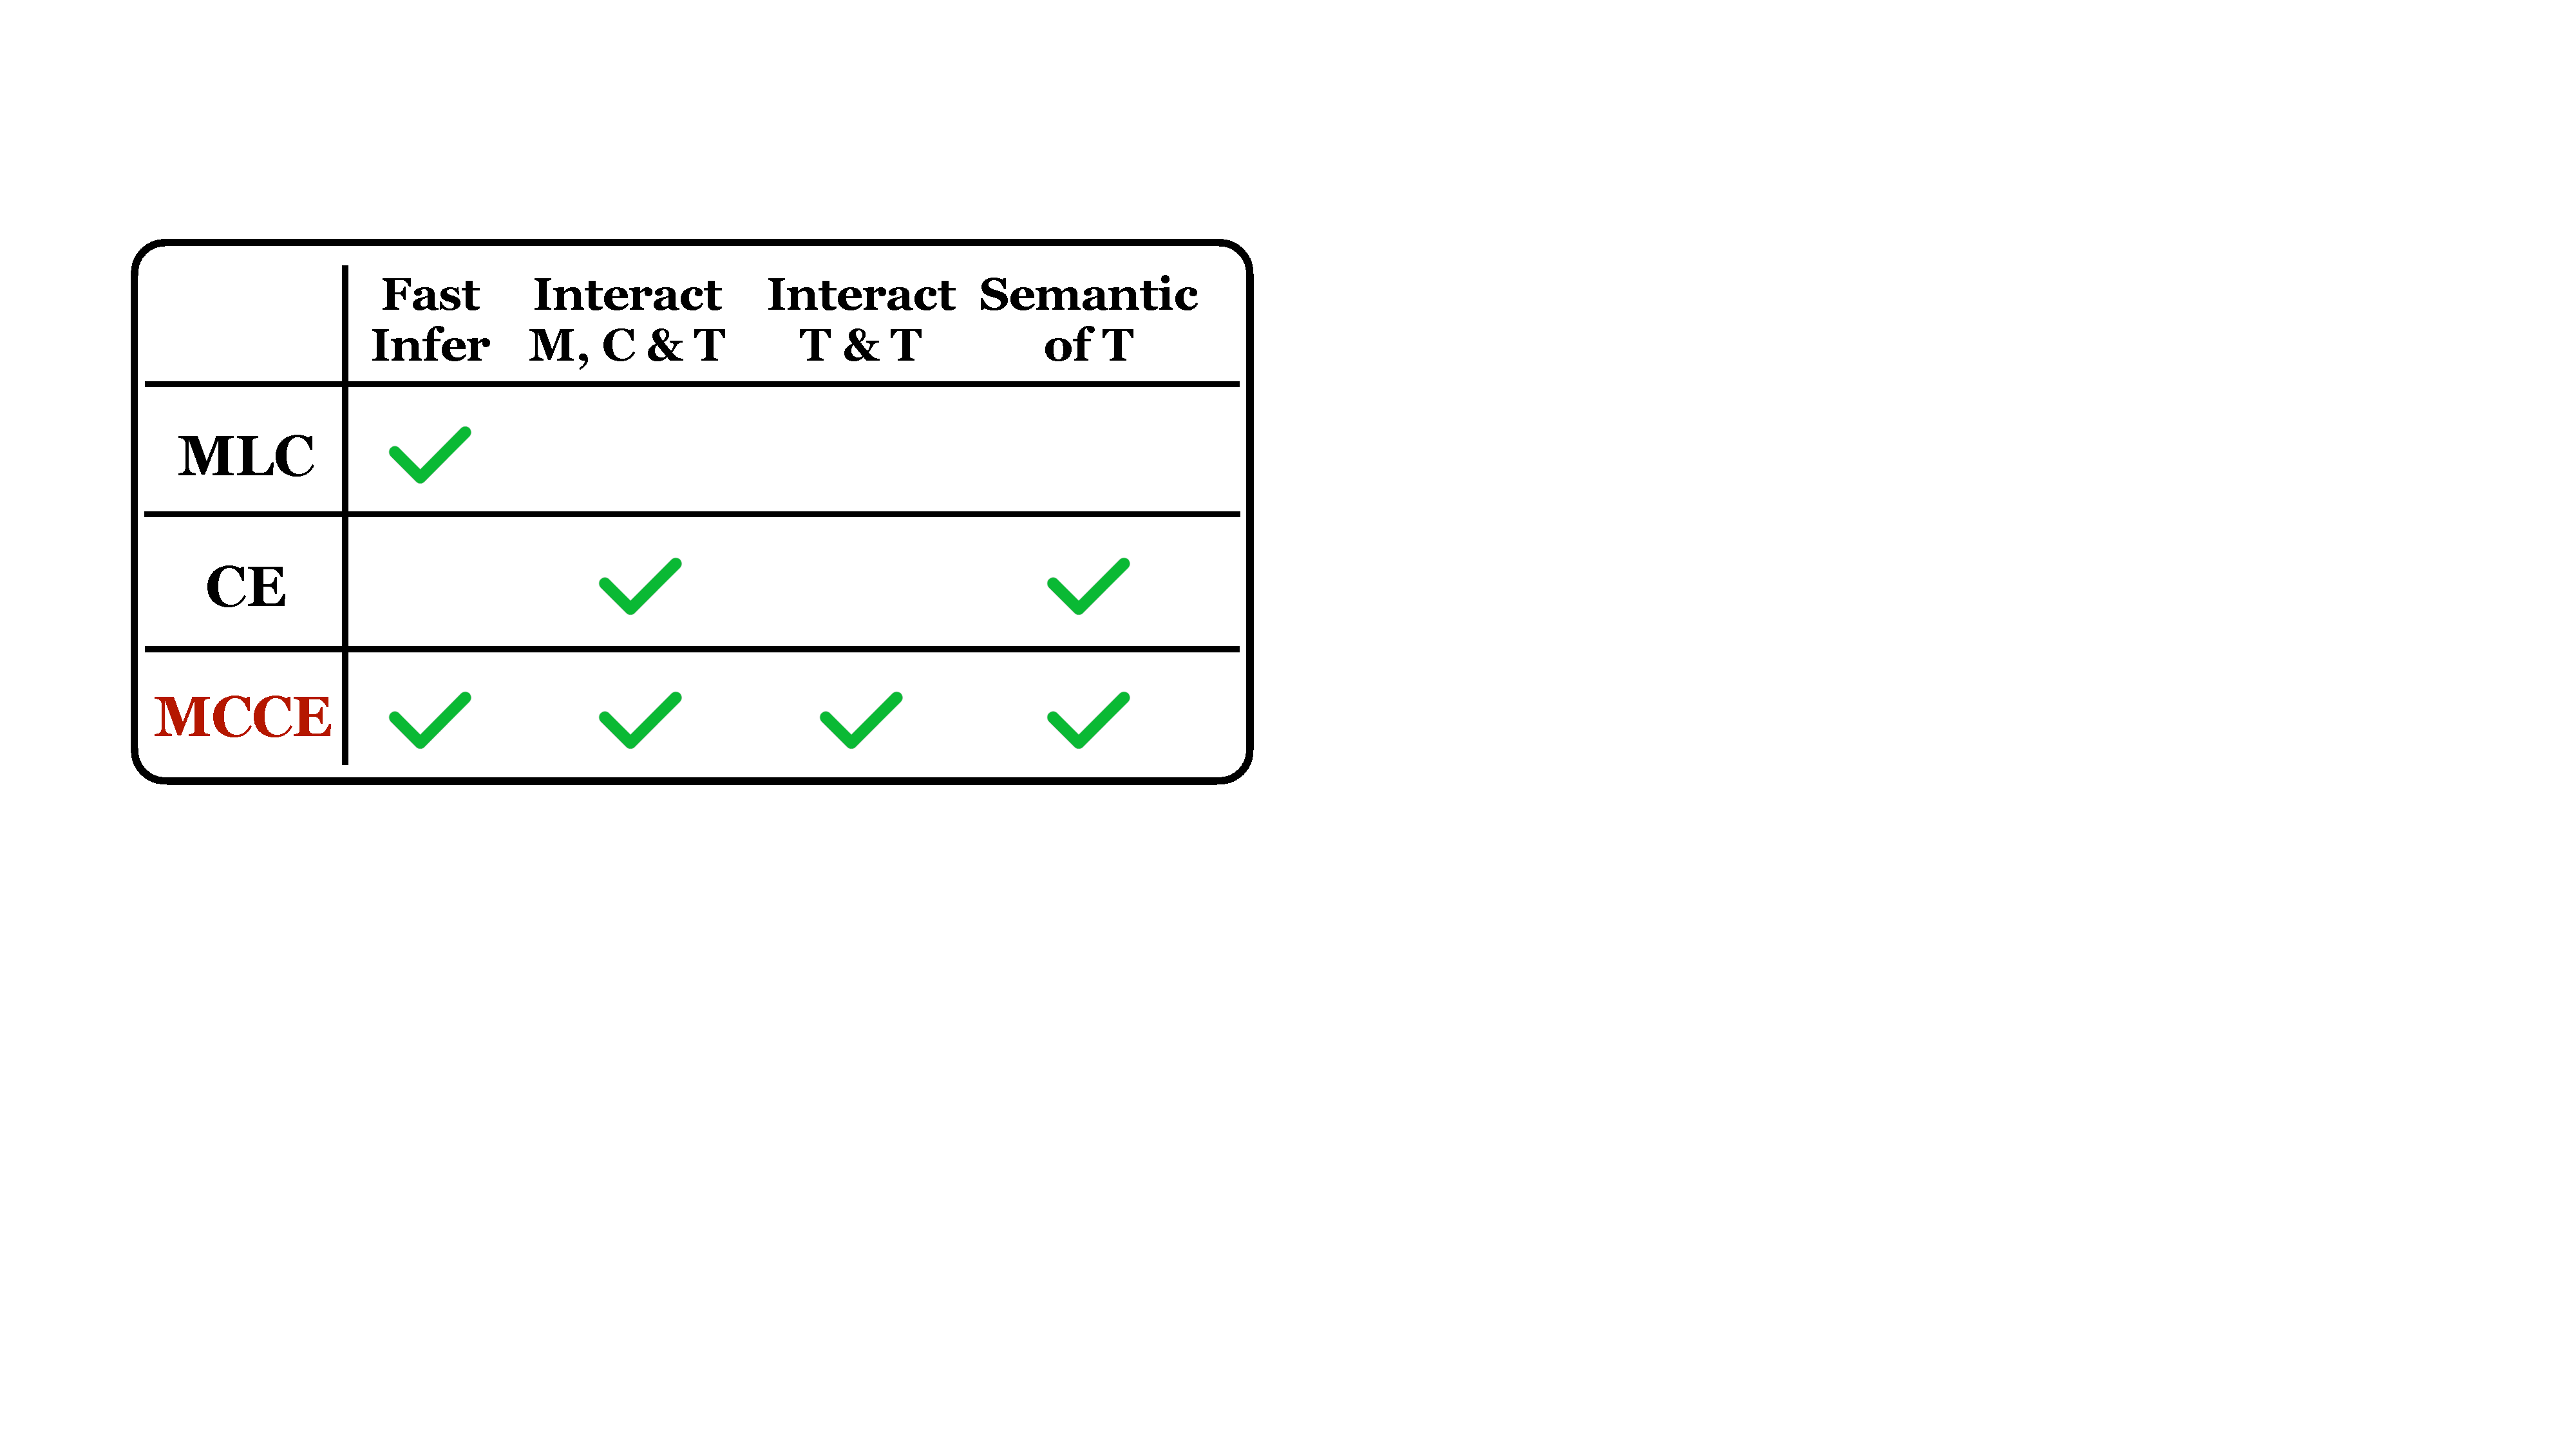
\includegraphics{src/img/adv.pdf}}
    \caption{Comparison of different models, M, C, and T are abbreviations of mention, context, and type.}
    \label{fig:adv}
\end{figure}

Experiments on two UFET datasets show that {\bf \textsc{\name}} and its variants under our recall-expand-filter paradigm reach SOTA performance and are thousands of times faster than the CE-based previous SOTA method. We also found {\bf \textsc{\name}} is still effective in fine-grained (130 types) and coarse-grained (9 types) entity typing. Our code is available at \code.
